% !TEX root = SystemTemplate.tex

\chapter{Overview and concept of operations}

This document will look at the We Don't Follow Directions team first sprint for building
a program tester. Looking at the team members and their roles, the project
management that we used, the sprint retrospective, any terminology or acronyms
that we use. Next we will look at the user stories, backlog and requirements of the
program. Then we will look at the design and implementation of the program focusing
on major pieces of the code. The next section will look at system and unit testing of 
our program, followed by development environment, and release, setup and
deployment of our program. We will finish this document with a look at a user 
documentation (including a user guide, installation guide and programmer manual)
class index and class documnetation.


\section{Scope}
This document will cover the first sprint of our program tester built for Dr. Logar's
software engineering class in Spring 2014 .


\section{Purpose}
To document the first sprint of the Software Engineering Program tester.


\subsection{Parse Directory Function}
Find the directory that we are looking for so we can traverse through it looking
for code to compile and run.

\subsection{Find Test Function}
Goes through the directory looking for source code to run, in order to compile
and test it.

\subsection{Run Difference Function}
This function will take in the output of the program we're testing and comparing it
with the expected output.

\section{Systems Goals}
The goal of this program is to run a program passed by command line, and test it
against found test cases. It will output if that test case passed or failed as well as
the totall cases passed, and total cases failed.

\section{System Overview and Diagram}
The program will be passed a source code file and compile and run that code.   To get test cases our
code will traverse a directory looking for .tst files.   It will use the test cases in the compiled code,
and output to a file.   That output file will be compared to the expected output file, if it passes we
write that test case to the log file and the passed or failed flag.   If we have used all the test cases
our program finishes by writing how many files passed, how many files failed, the percentages of
files that passed, and the percentage that failed, and close the program.   See Figure~\ref{systemdiagram}.

\begin{figure}[tbh]
\begin{center}
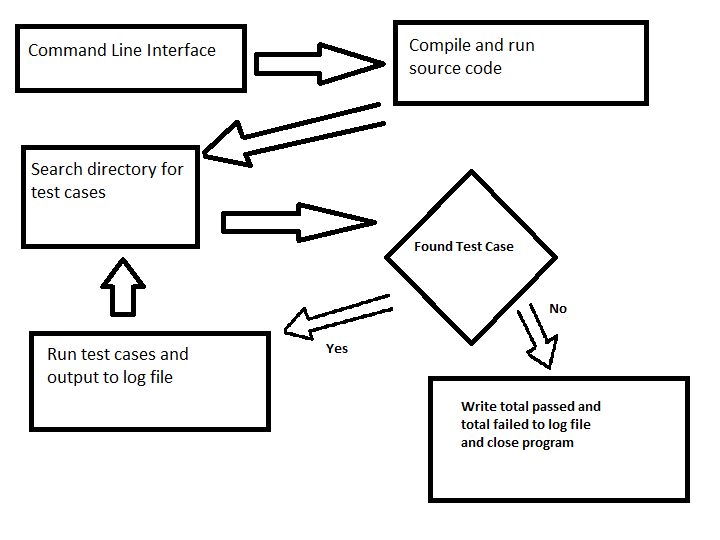
\includegraphics[width=0.75\textwidth]{./diagram}
\end{center}
\caption{System Diagram \label{systemdiagram}}
\end{figure}

\section{Technologies Overview}
We used C++ to write our code, in a Linux/GNU environment. We also used the system command to compile
and run the program we are testing, including the g++ compiler, and the diff function. We also used the iostream,
string, fstream, ctime, stdlib.h, dirent.h, and unistd.h libraries over the course of the program.

